\begin{figure*}[t]
    \centering
    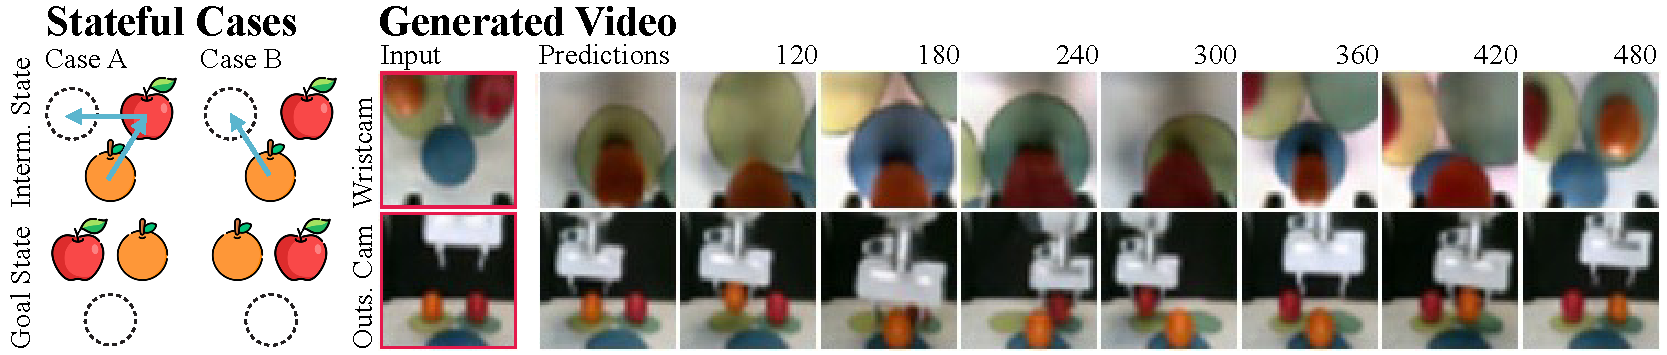
\includegraphics[width=\linewidth]{figures/pdf/Imitation.pdf}
    \caption{In our real robot task, a robot arm is asked to swap the slots of two fruits using a third slot. Since the fruits are input in random slots at the beginning, one cannot determine the next steps from a single observation without knowledge of the initial placement of the fruits. As illustrated in (a) and (b), the upper observation is the same but the desired outcome illustrated below can vary---the task thus requires remembering the initial configuration. In addition, as shown in (c), the same model that generates actions also synthesizes realistic video from just a single frame.}
    \label{fig:robot}
    \vspace{-10pt}
\end{figure*}
